\documentclass[11pt,fleqn]{article}
\usepackage[utf8]{inputenc}
\usepackage{graphicx}
\usepackage{amsmath}

%%%%%%%%%%%%%%%%%%%%%%%%%%%%%%%%%%%%%%%%%
%%% template that does not use Revtex4
%%% but allows special fonts
%%%%%%%%%%%%%%%%%%%%%%%%%%%%%%%%%%%%%%%%%


%%%%%%%%%%%%%%%%%%%%%%%%%%%%%%%%%%%%%%%%%%%
%%%
%%% Please use this template.
%%% Edit it using e.g. Notepad
%%% Ignore the header (do not change it)
%%% Process the file in the Latex site 
%%%
%%%%%%%%%%%%%%%%%%%%%%%%%%%%%%%%%%%%%%%%%%%


% Page setup
\topmargin -1.5cm      
\oddsidemargin -0.04cm   
\evensidemargin -0.04cm  
\textwidth 16.59cm
\textheight 24cm 
\setlength{\parindent}{0cm} 
\setlength{\parskip}{0cm} 


% Fonts
\usepackage{latexsym}
\usepackage{amsmath} 
\usepackage{amssymb} 
\usepackage{bm}


% Math symbols I
\newcommand{\sinc}{\mbox{sinc}}
\newcommand{\const}{\mbox{const}}
\newcommand{\trc}{\mbox{trace}}
\newcommand{\intt}{\int\!\!\!\!\int }
\newcommand{\ointt}{\int\!\!\!\!\int\!\!\!\!\!\circ\ }
\newcommand{\ar}{\mathsf r}
\newcommand{\im}{\mbox{Im}}
\newcommand{\re}{\mbox{Re}}

% Math symbols II
\newcommand{\eexp}{\mbox{e}^}
\newcommand{\bra}{\left\langle}
\newcommand{\ket}{\right\rangle}

% Mass symbol
\newcommand{\mass}{\mathsf{m}} 
\newcommand{\Mass}{\mathsf{M}} 

% More math commands
\newcommand{\tbox}[1]{\mbox{\tiny #1}}
\newcommand{\bmsf}[1]{\bm{\mathsf{#1}}} 
\newcommand{\amatrix}[1]{\begin{matrix} #1 \end{matrix}} 
\newcommand{\pd}[2]{\frac{\partial #1}{\partial #2}}

% Other commands
\newcommand{\hide}[1]{}
\newcommand{\drawline}{\begin{picture}(500,1)\line(1,0){500}\end{picture}}
\newcommand{\bitem}{$\bullet$ \ \ \ }
\newcommand{\Cn}[1]{\begin{center} #1 \end{center}}
\newcommand{\mpg}[2][1.0\hsize]{\begin{minipage}[b]{#1}{#2}\end{minipage}}
\newcommand{\Dn}{\vspace*{3mm}}

% Figures
\newcommand{\putgraph}[2][0.30\hsize]{\includegraphics[width=#1]{#2}}

% heading
\newcommand{\exnumber}[1]{\newcommand{\exnum}{#1}}
\newcommand{\heading}[1]{\begin{center} {\Large {\bf Ex\exnum:} #1} \end{center}}
\newcommand{\auname}[1]{\begin{center} {\bf Submitted by:} #1 \end{center}}


\begin{document} 
%%%%%%%%%%%%%%%%%%%%%%%%%%%%%%%%%%%%%%%%%%%%%%%%%%%%%%%%%%%%%%%%%%%%%%%%%%%%%%%%%%%%%%%%%%%%
%%%%%%%%%%%%%%%%%%%%%%%%%%%%%%%%%%%%%%%%%%%%%%%%%%%%%%%%%%%%%%%%%%%%%%%%%%%%%%%%%%%%%%%%%%%%
%%%%%%%%%%%%%%%%%%%%%%%%%%%%%%%%%%%%%%%%%%%%%%%%%%%%%%%%%%%%%%%%%%%%%%%%%%%%%%%%%%%%%%%%%%%%
%%%%%%%%%%%%%%%%%%%%%%%%%%%%%%%%%%%%%%%%%%%%%%%%%%%%%%%%%%%%%%%%%%%%%%%%%%%%%%%%%%%%%%%%%%%%
\exnumber{W10}
\heading{Hofstadter's butterfly}
\auname{Rotem Berman, Ori Yehezkel \& Ariel Falk }
\date{January 2020}
\graphicspath{{Images/}}
\setlength{\parindent}{0pt}

\section{The problem}
Consider a 2D square lattice with \math{3\times3}\endmath \space sites. Assume that the nearest neighbours hopping amplitude is c. Furthermore, assume that the magnetic flux through each plaque is \math{\Phi}. \endmath
\newline
\newline
Examine the following cases:
\begin{enumerate}
\item open boundary conditions.
\item periodic boundary condition in one axis and open boundary condition in the other.
\end{enumerate}
Write the Hamiltonian explicitly for both cases. Plot the eigenenergies as a function of the flux for a \math{15\times15}\endmath \space system. 




\section{The solution}


The problem consists of a 2D lattice formed of identical sites. The distance between two adjacent sites is a. The problem considers a case in which a particle can move between adjacent sites only, with hopping amplitude c. Let us use the position basis \math{|n,m>}\endmath \space where n, m denotes the x and y position of the site respectively. 
 
\begin{figure}[htp!]
\centerline
    {\includegraphics[scale=0.46]{5.jpg}}
    \caption{A schematic description of the system}
\end{figure}


\subsection{Open boundary conditions}

In the absence of a magnetic field the Hamiltonian of a \math{3\times3}\endmath \space site system, represented in the position basis, has the form:
$$H = \bordermatrix {
&|0,0>&|1,0>&|2,0>&|0,1>&|1,1>&|2,1>&|0,2>&|1,2>&|2,2>\cr
 &0&c&0&c&0&0&0&0&0\cr
 &c&0&c&0&c&0&0&0&0\cr
 &0&c&0&0&0&c&0&0&0\cr
 &c&0&0&0&c&0&c&0&0\cr
 &0&c&0&c&0&c&0&c&0\cr
 &0&0&c&0&c&0&0&0&c\cr
 &0&0&0&c&0&0&0&c&0\cr
 &0&0&0&0&c&0&c&0&c\cr
 &0&0&0&0&0&c&0&c&0}$$
\paragraph{}
When a homogeneous magnetic field,\space\math\vec{B}
\endmath,\space is applied in the \math\hat{z}\endmath\space direction, there is a magnetic flux \math{\Phi}\endmath \space through each plaque. 

Choosing the landau gauge for the vector potential:
 \begin{equation} \vec{A}=B(0,x,0)
 \end{equation}
 The accumulated phase between sites for motion in the x direction is zero while the accumulated phase for motion between sites in the y direction, \math{|n,m>,|n,m+1>}\endmath \space is: \begin{equation} \phi=\frac{e}{\hbar}\int\vec{A} d\vec{r}=\frac{e}{\hbar} \int_{am}^{a(m+1)}  Bx dy {=\frac{e}{\hbar}Bax=\frac{e}{\hbar}Ba^2n=\phi_0n} \end{equation}
defining \math{\phi_0\equiv \frac{e}{\hbar}Ba^2} \endmath. \newline \newline
 The x and y positions of the sites are discrete, where \math{x=na}\endmath , \math{y=ma} \endmath, \space \newline
 \math 0\leq n,m\leq N, \endmath \space and N is the number of sites in each axis. 
 Note that a circulation around any plaque contributes the same phase \math{\phi_0}\endmath. In addition, the magnetic flux through each plaque is \math{\Phi=Ba^2}\endmath.

\paragraph{}

The Hamiltonian of a \math{3\times3}\endmath \space sites represented in the position basis with the conditions described above is of the form:

$$
H = \bordermatrix {
&|0,0>&|1,0>&|2,0>&|0,1>&|1,1>&|2,1>&|0,2>&|1,2>&|2,2>\cr
 &0&c&0&c&0&0&0&0&0\cr
 &c&0&c&0&ce^{i\phi_0}&0&0&0&0\cr
 &0&c&0&0&0&ce^{2i\phi_0}&0&0&0\cr
 &c&0&0&0&c&0&c&0&0\cr
 &0&ce^{-i\phi_0}&0&c&0&c&0&ce^{i\phi_0}&0\cr
 &0&0&ce^{-2i\phi_0}&0&c&0&0&0&ce^{2i\phi_0}\cr
 &0&0&0&c&0&0&0&c&0\cr
 &0&0&0&0&ce^{-i\phi_0}&0&c&0&c\cr
 &0&0&0&0&0&ce^{-2i\phi_0}&0&c&0}
$$
\paragraph{}
By numerically diagonalizing the Hamiltonian of a \math{15\times15}\endmath \space system, we obtain the energy spectrum as a function of \math{\Phi} \endmath:




\begin{figure}[htp!]
\centerline
    {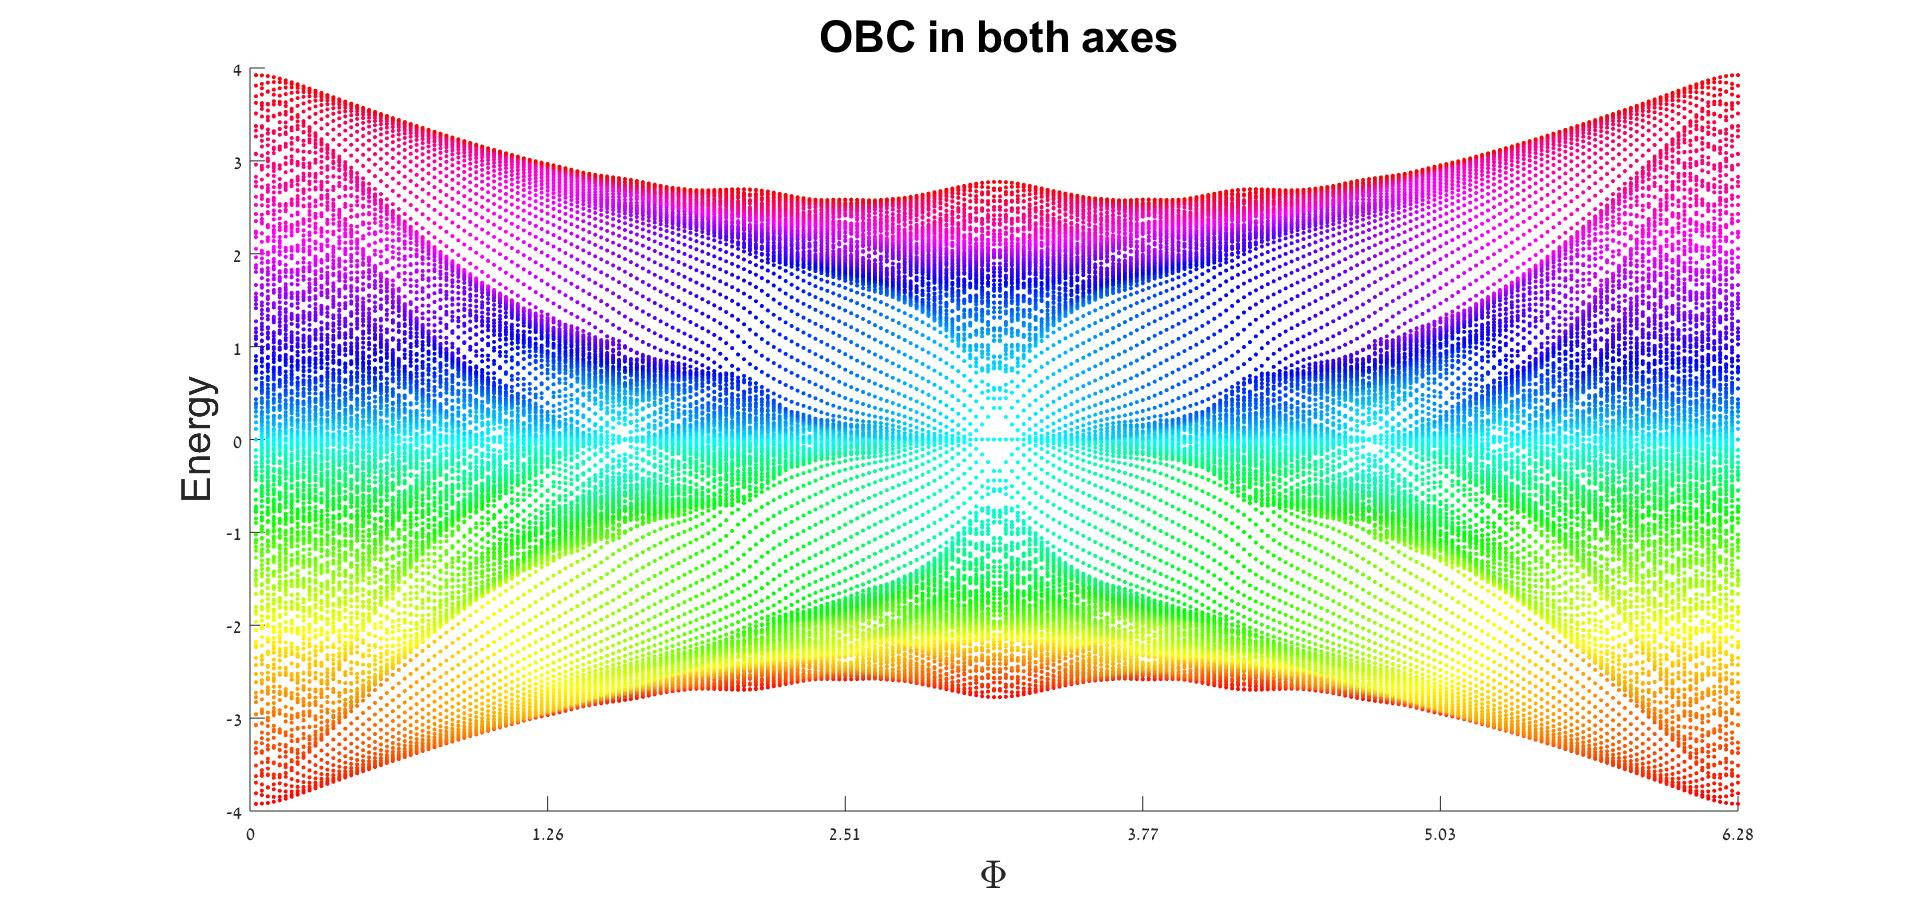
\includegraphics[scale=0.25]{OBCinbothaxes15sites.jpg}}
    \caption{The energy spectrum of a \math{15\times15}\endmath\space site system with OBC in both axes.}
\end{figure}
 







\subsection{Periodic boundary conditions in the x axis}
Upon adding periodic boundary condition in the x axis and using the same gauge as used before, there will be no accumulated phase in the x axis. The calculation of the phase accumulated in the y axis is as presented before.

Under these conditions the Hamiltonian is:
\paragraph{}
$$
H = \bordermatrix {
&|0,0>&|1,0>&|2,0>&|0,1>&|1,1>&|2,1>&|0,2>&|1,2>&|2,2>\cr
 &0&c&c&c&0&0&0&0&0\cr
 &c&0&c&0&ce^{i\phi_0}&0&0&0&0\cr
 &c&c&0&0&0&ce^{2i\phi_0}&0&0&0\cr
 &c&0&0&0&c&c&c&0&0\cr
 &0&ce^{-i\phi_0}&0&c&0&c&0&ce^{i\phi_0}&0\cr
 &0&0&ce^{-2i\phi_0}&c&c&0&0&0&ce^{2i\phi_0}\cr
 &0&0&0&c&0&0&0&c&c\cr
 &0&0&0&0&ce^{-i\phi_0}&0&c&0&c\cr
 &0&0&0&0&0&ce^{-2i\phi_0}&c&c&0
}
$$

\paragraph{}
As before, diagonalizing the hamiltonian of a \math{15\times15}\endmath\space system yields the following energy spectrum as a function of \math{\Phi} \endmath:

\begin{figure}[htp!]
\centerline
    {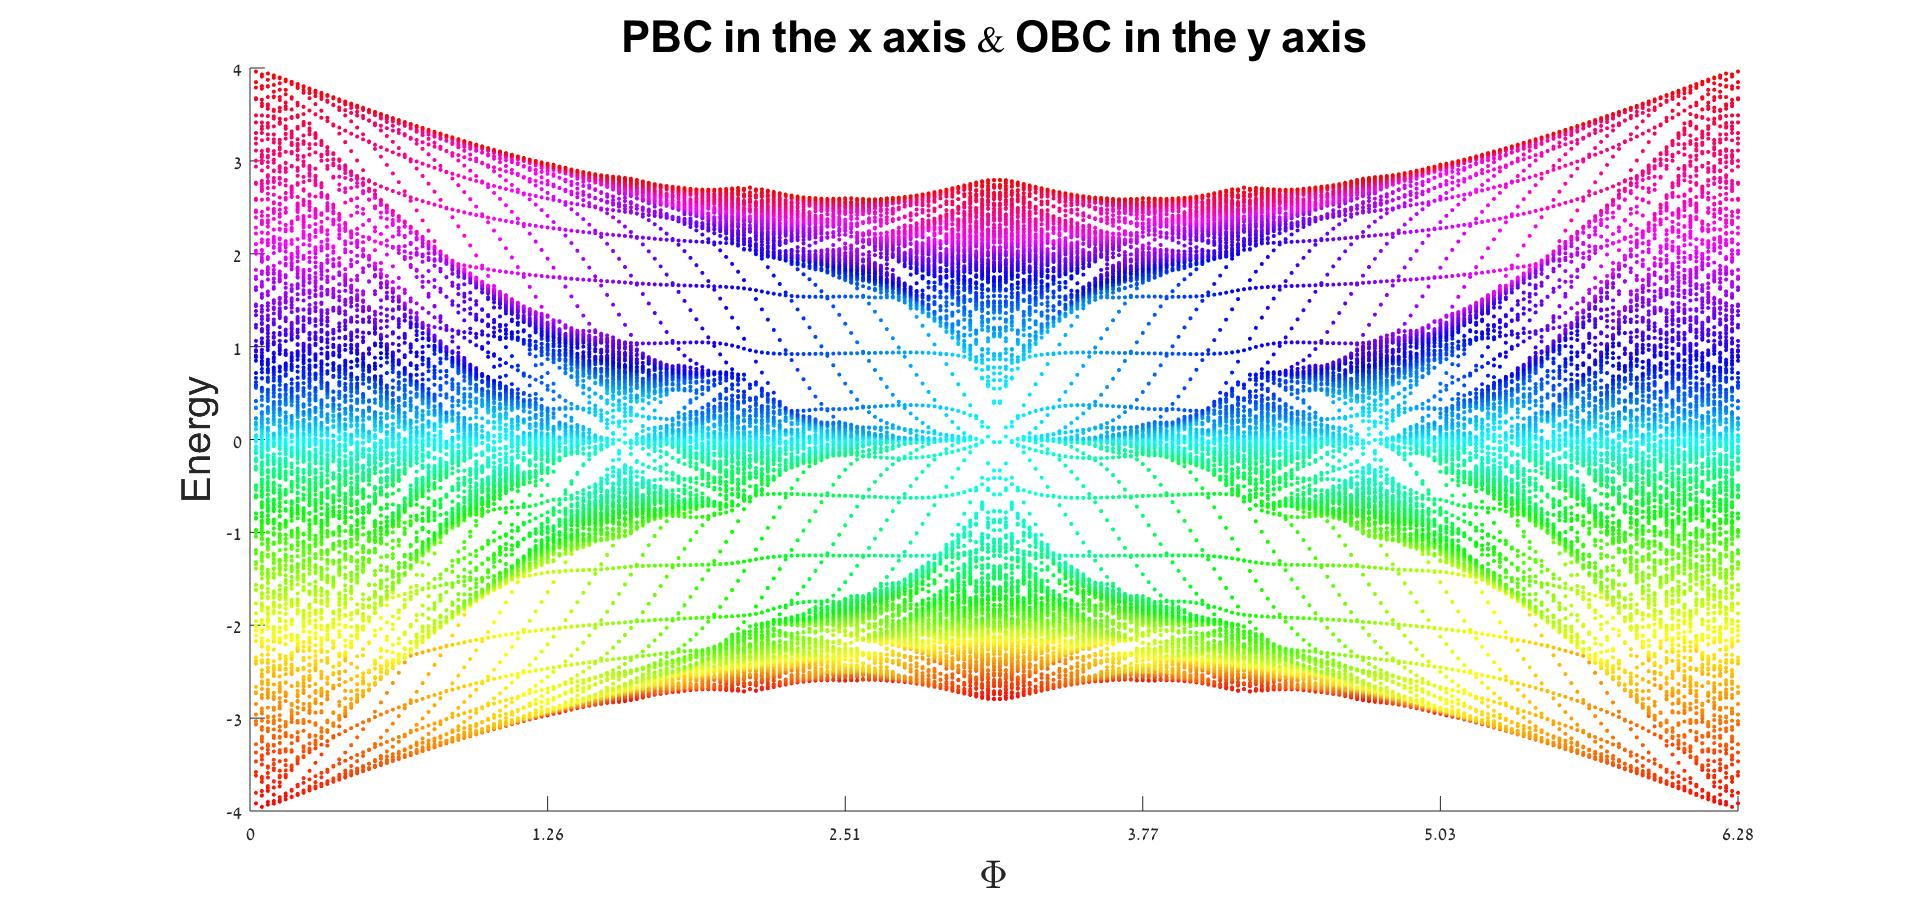
\includegraphics[scale=0.25]{2.jpg}}
    \caption{The energy spectrum of a \math{15\times15}\endmath\space sites system with PBC in the x axis and OBC in the y axis}
\end{figure}

\end{document}




